\chapter{Correctness}
\paragraph{}In this section, we show that, once topology changes cease, the algorithm eventually terminates with each connected component being leader-oriented. As a result, the $lid_u$ variables satisfy the conditions of the leader election problem.
\paragraph{}We first show, in Section 4.1, an important relationship between the final communication topology and the forming and $N$ variables of the nodes. The rest of the proof uses a number of invariants, denoted as “Properties”, which are shown to hold in every configuration of every execution; each one is proved (separately) by induction on the configurations occurring in an execution. In Section 4.2, we introduce some definitions and basic facts regarding the information about nodes' heights that appears in the system, either in nodes' height arrays or in messages in transit. In Section 4.3, we bound, in Lemma 3, the number of elections that can occur after the last topology change; this result relies on the fact, shown in Lemma 2, that once a node $u$ adopts a leader that was elected after the last topology change, $u$ never becomes a sink again. Then in Section 4.4, we bound, in Lemma 4, the number of new reference levels that are started after the last topology change; the proof of this result relies on several additional properties. Section 4.5 is devoted to showing, in Lemmas 5, 6, and 7, that eventually there are no messages in transit and every node has an accurate view of its neighbors' heights. All the pieces are put together in Theorem 1 of Section 4.6 to show that eventually we have a leader-oriented connected component; a couple of additional properties are needed for this result.
\paragraph{}Throughout the proof, consider an arbitrary execution of the algorithm in which the last topology change event occurs at some global time $t_{LTC}$, and consider any connected component of the final topology.
\section{Channels and Neighbors}
\paragraph{}Because of the lack of coordination between the topology change events for the two channels going between nodes $u$ and $v$ in the two directions, $u$ and $v$ do not necessarily have consistent views of their local neighborhoods in $G_{chan}$, even after the last topology change. For instance, it is possible that $v$ is in $N_u$ but $u$ is not in $N_v$ forever after the last topology change. Suppose the channel from $u$ to $v$ remains $Up$ from some time $t$ onwards, so that $v$ remains in $N_u$ from time $t$ onwards. However, suppose that the channel from $v$ to $u$ fluctuates several times after time $t$, eventually stabilizing to being $Up$ (cf. Fig. 5). Every time the channel to $u$ goes down, $u$ is removed from $v$'s forming and $N$ sets. Every time the channel to $u$ comes up, $v$ adds $u$ to $forming_v$ and sends its height in an $Update$ message to $u$. When $u$ gets the message from $v$, it updates the entry for $v$ in its height array, but does not send its own height back to $v$. As long as $u$'s height does not change, $u$ does not send its height to $v$. Thus $v$ is never able to move $u$ from $forming_v$ into $N_v$.
\begin{figure}[h]
	\centering
	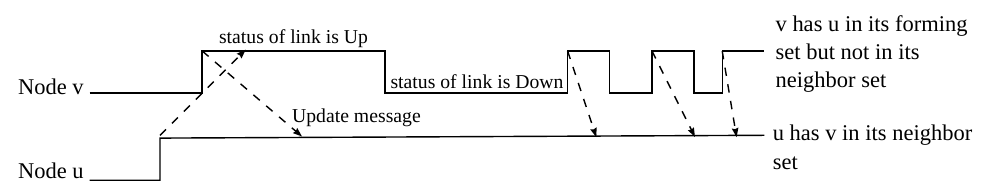
\includegraphics[width=1\linewidth]{fig_1}
	\caption[The status of the channel from $u$ to $v$ remains $Up$, but the status of the channel from $v$ to $u$ fluctuates.]{The status of the channel from $u$ to $v$ remains $Up$, but the status of the channel from $v$ to $u$ fluctuates.}
	\label{fig:fig1}
\end{figure}
\paragraph{}However, we are assured by Lemma 1 below that after time $t_{LTC}$ , $N_u \cup forming_u$ does not change for any node $u$. Furthermore, a node $u$ always sends $Update$ messages to all nodes in $N_u \cup forming_u$ , which constitutes all the outgoing channels of $u$.
\paragraph{Lemma 1}After time $t_{LTC}$, $N_u \cup forming_u$ does not change for any node $u$.
\subparagraph{Proof}When $ChannelDown_{uv}$ occurs, $u$ removes $v$ from both its $N_u$ and $forming_u$ variables. When $ChannelUp_{uv}$ occurs, $u$ adds $v$ to its $forming_u$ variable and sends an $Update$ message to $v$. When $u$ receives an $Update$ message from a node $v$, the only possible change to the $N_u$ and $forming_u$ variables is that $v$ is moved from $forming_u$ to $N_u$, which does not change $N_u \cup forming_u$.
\subparagraph{}$t_{TLC}$ is the latest among all the times at which either a $ChannelDown$, or a $ChannelUp$ occurs. After this time, the only change to the $N$ set or the forming set must be due to receipt of an $Update$ message, causing lines 2 and 3 of Figure 2 to be executed. Thus the only change to the $N$ set or the forming set is that a node which is removed from the forming set is added to the $N$ set. This does not affect $N \cup forming$.
\section{Height Tokens and Their Properties}
\paragraph{}Since a node makes algorithm decisions based solely on comparisons of its neighboring nodes' height tuples, we first present several important properties of the tuple contents. Define $h$ to be a height token for node $u$ in a configuration if $h$ is in an $Update$ message in transit from $u$, or $h$ is the entry for $u$ in the height array of any node. Let $LP(h)$ be the leader pair of $h$, $RL(h)$ the reference level (triple) of $h$, $\delta(h)$ the $\delta$ value of $h$, $lts(h)$ the absolute value of the (non-positive) leader timestamp (component $nlts$) of $h$, and $\tau (h)$ the $\tau$ value of $h$.
\paragraph{}Given a configuration in which $Channel(u, v)$ has status $Up$ and $u \in N_v$ , the $(u, v)$ height sequence is defined as the sequence of height tokens $h_0, h_1, ... , h_m$, where $h_0$ is $u$'s height, $h_m$ is $v$'s view of $u$'s height, and $h_1, ..., h_{m-1}$ is the sequence of height tokens in the $Update$ messages in transit from $u$ to $v$. If the status of $Channel(u, v)$ is $Up$ but $u \not\in N_v$ , then the $(u, v)$ height sequence is defined similarly except that $h_1, ... , h_m$ is the sequence of height tokens in the $Update$ messages in transit from $u$ to $v$; in these cases, $v$ does not have an entry for $u$ in its height array. If $Channel(u, v)$ is $Down$, the $(u, v)$ height sequence is undefined.
\paragraph{Property A}If $h$ is a height token for a node $u$ in the $(u, v)$ height sequence, then:
\begin{enumerate}
	\item $lts(h) \leq \mathcal{T} _u$ and $\tau (h) \leq \mathcal{T} _u$
	\item If $h$ is in $v$'s height array then $lts(h) \leq \mathcal{T} _v$ and $\tau (h) \leq \mathcal{T} _v$ .
\end{enumerate}
\newpage

\subparagraph{Proof}By induction on the configurations in the execution.
\subparagraph{}\textit{Basis:} In the initial configuration $C_0$ , all the leader timestamps and $\tau$ values are $0$ and $\mathcal{T} \geq 0$ for all nodes $v$.
\subparagraph{}\textit{Inductive Hypothesis:} Suppose the property is true in configuration $C_{i-1}$ and show it remains true in configuration $C_i$. Since the property is true in $C_{i-1}$ , for every height token $h$ in the $(u, v)$ height sequence, we have:
\begin{enumerate} [label=(\roman*)]
	\item $lts(h) \leq \mathcal{T} _u(C_{i-1})$ and $\tau (h) \leq \mathcal{T} _u(C_{i-1})$
	\item If $h$ is in $v's$ height array then $lts(h)$ $\leq$ $\mathcal{T} _v(C_{i-1})$ and $\tau (h)$ $\leq$ $\mathcal{T} _v (C_{i-1})$
\end{enumerate}
\subparagraph{}\textit{Inductive Step:} If $h$ is a preexisting height token during event $e_i$ (the event immediately preceding $C_i$), then by the inductive hypothesis and the increasing property of $\mathcal{T} _u$, it follows that $lts(h) \leq \mathcal{T} _u (C_i)$ and $\tau (h) \leq \mathcal{T} _u(C_i)$. If, on the other hand, $h$ is created during event $e_i$, then any new values of $lts$ and $\tau$ generated by $u$ are equal to $\mathcal{T} _u(C_i)$ and, thus, the property remains true.
\subparagraph{}If $h$ is a height token for node $u$ at some other node $v$, then $h$ was either present at $v$ during $C_{i-1}$ or was received at $v$ during event $e_i$, immediately preceding $C_i$. In the first case, by the inductive hypothesis and the increasing property of $\mathcal{T} _v$, it follows that $lts(h) \leq \mathcal{T} _v (C_i)$ and $\tau (h) \leq \mathcal{T} _v (C_i)$. In the second case, there exists a message through which $v$ received $h$ from $u$ during event $e_i$ . Since $\mathcal{T}$ preserves causality, by the definition of the happens before relation, it follows that the creation of either $\tau (h)$ or $lts(h)$ preceded the receipt of the message by $v$. Therefore, in configuration $C_i$ it remains true that $lts(h) \leq \mathcal{T} _v (C_i)$ and $\tau (h) \leq \mathcal{T} _v (C_i)$.
\paragraph{}Property B, given below, states some important facts about height sequences. If the channel's status is $Up$ and $m = 1$, meaning that no messages are in transit from $u$ to $v$, then Part (1) of Property B indicates that $v$ has an accurate view of $u$'s height. If there are $Update$ messages in transit, then the most recent one sent has accurate information. Part (2) of Property B implies that leader pairs are taken on in decreasing order. Part (3) of Property B implies that reference levels are taken on in increasing order with respect to the same leader pair. Note that Property B only holds if $m > 0$.
\paragraph{Property B:}Let $h_0, h_1, ... , h_m$ be the $(u, v)$ height sequence for any $Channel(u, v)$ whose status is $Up$. Then the following are true if $m > 0$:
\begin{enumerate}
	\item $h_0 = h_1$.
	\item For all $l$, $0 \leq l < m,~LP(h_l ) \leq LP(h_{l+1} )$.
	\item For all $l$, $0 \leq l < m,$ if $LP(h_l ) = LP(h_{l+1})$, then $RL(h_l) \geq RL(h_{l+1})$.
\end{enumerate}
\paragraph{Proof}The proof is by induction on the execution.
\subparagraph{}Initially in $C_0$, $Channel(u, v)$ is either $Up$ or $Down$. If $Channel(u, v)$ is $Down$, then the $(u, v)$ height sequence is undefined. If $Channel(u, v)$ is $Up$, then the definition of initial configurations states that no messages are in transit and $v$ has an accurate view of $u$'s height, that is, $m = 1$ and $h_0 = h_1$.
\subparagraph{}Suppose the property is true in configuration $C_{i-1}$ and show it is still true in configuration $C_i$.
\subparagraph{}Suppose event $e_i$ is $ChannelDown_{uv}$. Then the $(u, v)$ height sequence is not defined in $C_i$.
\subparagraph{}Suppose event $e_i$ is $ChannelUp_{uv}$. By the assumption that the channel up/down events for a given channel alternate, the state of the channel in $C_{i-1}$ is Down and there are no messages in transit. Thus in $C_i$ the $(u, v)$ height sequence is $h$, where $h$ is the height of $u$ in $C_i$, which is stored in $u's$ height array and is in the $Update$ message that $u$ sends to $v$. Clearly this height sequence satisfies the three conditions.
\subparagraph{}Suppose event $e_i$ is the receipt by $v$ of an $Update$ message from $u$. In one case, the $(u, v)$ height sequence changes by dropping the last element, if the oldest message in transit takes the place of $v's$ view of $u's$ height. In the other case, the $(u, v)$ height sequence does not change if the receipt causes $v$ to record $u's$ height and add $u$ to $N_v$. In both cases, the three conditions still hold.
\subparagraph{}Suppose event $e_i$ is the receipt by $u$ of an $Update$ message from node $w$ or is a $ChannelDown$ event for a channel to some node other than $v$. If $u$ does not change its height, then there is no change affecting the property.
\subparagraph{}Suppose $u$ changes its height from $h' _0$ to $h$.
\subparagraph{}Let the $(u, v)$ height sequence in $C_{i-1}$ be $h' _0 , h'_1, ... , h'_m$. By the inductive hypothesis, $h' _0 = h' _1$ . By the code, the $(u, v)$ height sequence in $C_i$ is $h, h, h'_1 , ... , h'_m$. In each case we just have to show that $h$ has the proper relationship to $h'_1$, which equals $h'_0$.
\subparagraph{}Case 1: $e_i$ calls $REFLECTREFLEVEL$: All of $u's$ neighbors are viewed as having the same $LP$ as $u$, having reference level $(t, p, 0)$ for some $t$ and $p$, and having a larger height than $u$.
\subparagraph{}Since $u$ is a sink during the step, $RL(h'_0 )$ $\leq$ $(t, p, 0)$. Since $RL(h) = (t, p, 1)$, and the old and new $LP$ are the same, the property holds.
\subparagraph{}Case 2: $e_i$ calls $ELECTSELF$: By Property A, $lts$ in $LP(h'_0 )$ is less than or equal to $\mathcal{T} _{u'}$ in configuration $C_{i-1}$. The new leader pair has $lts~\mathcal{T} _u$ in configuration $C_i$, which is greater than $\mathcal{T} _{u'}$. So $LP(h)$ $\leq$ $LP(h'_0 )$.
\subparagraph{}Case 3: $e_i$ calls $STARTNEWREFLEVEL$: By Property A, the $\tau$ value in $RL(h'_0 )$ is less than or equal to $\mathcal{T}_u'$ at configuration $C_{i-1}$. The new reference level has $\tau$ value $\mathcal{T}_u$ at configuration $C_i$, which is greater than $\mathcal{T}_{u'}$ and the $LP$ is unchanged. So $LP(h) = LP(h'_0 )$ and $RL(h)$ $\geq$ $RL(h'_0 )$.
\subparagraph{}Case 4: $e_i$ calls $PROPAGATELARGESTREFLEVEL$: All neighbors of $u$ are viewed as having the same $LP$ as $u$, but with different $RLs$ among themselves, and as having larger heights than $u$. By the code, $u$ takes on the largest neighboring $RL$, which is at least as large as $u's$ old $RL$, since $u$ is a sink. The $LP$ is unchanged. So $LP(h) = LP(h'_0 )$ and $RL(h)$ $\geq$ $RL(h'_0 )$.
\subparagraph{}Case 5: $e_i$ calls $ADOPTLPIFPRIORITY$: By the code, the new $LP$ is smaller than the previous, so $LP(h) < LP(h'_0 )$.
\newpage
\section{Bounding the Number of Elections}
\paragraph{}In this subsection, we show that every node elects itself at most a finite number of times after the last topology change.
\paragraph{}Define the following with respect to any configuration in the execution. For $LP (-s, l)$, where $\mathcal{T}_l (t) = s$ and $t$ $\geq$ $t_{LTC}$, let $LP$ tree $LT (-s, l)$ be the sub-graph of the connected component whose vertices consist of all nodes that have taken on $LP (-s, l)$ in the execution (even if they no longer have that $LP$), and whose directed edges are all ordered pairs $(u, v)$ such that $v$ adopts $LP (-s, l)$ due to the receipt of an $Update$ message from $u$. Since a node can take on a particular $LP$ only once by Property B, $LT (-s, l)$ is a tree rooted at $l$.
\paragraph{Porperty C:}For each height token $h$ with $RL (t, p, r)$, either $t = p = r = 0$, or $t > 0$, $p$ is a node $id$, and $r$ is $0$ or $1$.
\subparagraph{Proof}The proof is by induction on the sequence of configurations in the execution. The basis follows since all height tokens in an initial configuration have $RL (0, 0, 0)$.
\subparagraph{}For the inductive step, we consider all the ways that a new $RL$ can be generated (as opposed to copying an existing one). In $ELECTSELF$, the new $RL$ is $(0,0,0)$. In $STARTNEWREFLEVEL$ , the new RL is $(t, p, 0)$, where $t$ is the current causal clock time, which is positive, and $p$ is a node $id$. In $REFLECTREFLEVEL$, the new $RL$ is $(t, p, 1)$, where $(t, p, 0)$ is a preexisting height token. By the precondition for executing $REFLECTREFLEVEL$, $t$ is positive. By the inductive hypothesis applied to the preexisting height token $(t, p, 0)$, $p$ is a node $id$.
\paragraph{Property D:}Let $h$ be a height token for some node $u$. If $LP(h) = (-s, l)$, where for some global time $t$, $T_l (t) = s$ and $t \geq t_{LTC}$ , then $RL(h) = (0, 0, 0)$ and $\delta (h)$ is the distance in $LT (-s, l)$ from $l$ to $u$.
\subparagraph{Proof:}By induction on the sequence of configurations in the execution.
\subparagraph{}By Property A, the basis is configuration $C_j$, just after the event at global time $t$ when the first height tokens with $LP (-s, l)$ are created. By the code, these height tokens are created by node $l$ for itself and have $RL (0, 0, 0)$ and $\delta = 0$.
\subparagraph{}Assume the property is true in configuration $C_{i-1}$ , with $i-1$ $\geq$ $j$, and show it is true in configuration $C_i$. Since no further topology changes occur, the only possibility for event $e_i$ is the receipt of an $Update$ message. Suppose node $u$ receives $Update(h)$ from node $v$.
\subparagraph{}As a result of the receipt of the message, $u$ records $h$ as $v$'s height in its view. The inductive hypothesis implies that the property remains true for this new height token.
\subparagraph{}Also as a result of the receipt of the message, $u$ might change its height.
\subparagraph{}Suppose $u$ changes its height by executing $ADOPTLPIFPRIORITY$, adopting the $LP$ in $h$, where $LP(h) = (-s, l)$. By the inductive hypothesis, $RL(h) = (0, 0, 0)$, and $\delta (h)$ is the distance from $l$ to $v$ in $LT (-s, l)$ in $C_{i-1}$. By Property B, since $u$ adopts $(-s, l)$, it must be that $u's$ $LP$ is larger than $(-s, l)$ in $C_{i-1}$ , and thus $v$ is $u's$ parent in $LT (-s, l)$. By the code, $u$ sets its $RL$ to $(0, 0, 0)$ and its $\delta$ to $\delta (h) + 1$. But this is exactly the distance in $LT (-s, l)$ from $l$ to $u$. So all height tokens created in this step satisfy the property.
\subparagraph{}Suppose $u$ changes its height because it becomes a sink and $u's$ new height has $LP (-s, l)$. First, we show that $u$ does not take on $LP (-s, l)$ as a result of $ELECTSELF$. By assumption, $LP (-s, l)$ is created in configuration $C_j$ (the base case). By the code and the increasing property of causal clocks, it follows that $l$ cannot create a duplicate of $LP (-s, l)$ at some later configuration $C_i$. Therefore, $u$ does not take on $LP (-s, l)$ as a result of $ELECTSELF$.
\subparagraph{}Thus, the old height of $u$, call it $h'$, also has $LP (-s, l)$. Since $u$ becomes a sink, all its neighbors have $LP (-s, l)$ in $u's$ view, and by the inductive hypothesis they all have $RL (0, 0, 0)$ in $u's$ view. Thus the new height of $u$ is not the result of executing $REFLECTREFLEVEL$ (which requires the neighbors' common $\tau$ to be positive) or $PROPAGATELARGESTREFLEVEL$ (which requires the neighbors to have different $RL's$). Instead, it must be the result of executing $STARTNEWREFLEVEL$. Since $u$ is a sink and $(0, 0, 0)$ is the smallest possible $RL$ by Property C, $RL(h' ) = (0, 0, 0)$. Also, since $u$ is a sink, $u = l$. Let $v$ be $u's$ parent in the $LP-tree~LT (-s, l)$ and let $d$ be the distance in that tree from $l$ to $v$. By the inductive hypothesis, in $u's$ view of $v's$ height, $v's$ $\delta = d$, but in $u's$ own height, $\delta = d + 1$. Thus the edge between $u$ and $v$ is directed toward $v$, and $u$ cannot be a sink, a contradiction.
\paragraph{Lemma 2}Any node $u$ that adopts leader pair $(-s, l)$ for any $l$ and any $s$, where for some global time $t$, $\mathcal{T}_l (t) = s$ and $t > t_{LTC}$ , never subsequently becomes a sink.
\subparagraph{Proof}Suppose in contradiction that $u$ adopts leader pair $(-s, l)$ at global time $t_1 > t$ and that at global time $t_2 > t_1$, $u$ becomes a sink. Suppose $u$ does not change its leader pair in the time interval $(t_1 ,t_2 )$. (If $u$ did change its leader pair, the new leader pairs would all be smaller than $(-s, l)$ by Property B, and the argument would still hold with respect to the latest leader pair taken on by $u$ in that time interval.)
\subparagraph{}Let $v$ be the parent of $u$ in the $LP$-tree $LT(-s, l)$. Immediately after time $t_1$, the link $(u, v)$ is directed from $u$ to $v$ in $u's$ view.
\subparagraph{}In order for $u$ to become a sink at time $t_2$ , there must be some time between $t_1$ and $t_2$ when the link $(u, v)$ reverses direction in $u's$ view. Suppose the link reverses because $u's$ height lowers. Recall that $u$ does not change its leader pair in $(t_1,t_2 )$ by assumption. By Property D, $u's$ reference level remains $(0, 0, 0)$ in $(t_1 ,t_2 )$ and $u's$ $\delta$ stays the same in the interval. That is, $u's$ height does not change, and in particular does not lower. Thus the only way that the link $(u, v)$ can reverse direction in $(t_1 ,t_2 )$ is due to the receipt by $u$ of an update message from $v$ with a new height for $v$ that is higher than $u's$ height.
\subparagraph{}How can $v's$ height change after $v$ takes on leader pair $(-s, l)$ ? One possibility is that $v's$ leader pair changes. By Property B, any change in $v's$ leader pair will be to a smaller one, which will be adopted by $u$ together with a $\delta$ value that keeps the link directed from $u$ to $v$ in $u's$ view.
\subparagraph{}The other possibility is that $v$'s leader pair does not change but some other component of its height changes. But by Property D, since $v$'s leader pair has timestamp $-s$ with $\mathcal{T} _l (t) = s$ and $t > t_{LTC}$ , $v$'s RL and $\delta$ cannot change.
\subparagraph{}Thus no change to $v's$ height reported to $u$ after time $t_1$ can cause the link $(u, v)$ to be directed from $v$ to $u$ in $u's$ view, and $u$ cannot be a sink at time $t_2$ , which is a contradiction.
\paragraph{Lemma 3}No node elects itself more than a finite number of times after global time $t_{LTC}$.
\subparagraph{Proof}Suppose in contradiction that a node $u$ elects itself an infinite number of times after the last topology change. Once it has elected itself the first time, the only way it can become a sink and elect itself again is by adopting a new $LP$ first. Thus, node $u$ needs to adopt new $LP's$ infinitely often after $t_{LTC}$ . By Property B, the leader timestamp of each subsequent $LP$ has to be greater than the previous one, which results in an increasing sequence of leader timestamps that $u$ adopts. Let $\mathcal{T}_{max}$ be the maximum of the clocks of all nodes at time $t_{LTC}$. In the process of adopting increasing leader timestamps, at some point $u$ will adopt $LP(-s, l)$ where $\mathcal{T} _l (t) = s$ and for which $s > \mathcal{T} _{max}$.
\subparagraph{}This follows from the first property of causal clocks which states that for each node $u$, the values of $\mathcal{T}_u$ are increasing, i.e., if $e_i$ and $e_j$ are events involving $u$ in the execution with $i < j$, then $\mathcal{T} _u (e_i ) < \mathcal{T} _u (e_j )$, and, furthermore, if there is an infinite number of events involving $u$, then $\mathcal{T} _u$ increases without bound. 
\subparagraph{}Because $\mathcal{T} _{max}$ was the maximum value of all clocks at the time of the last topology change, it follows that $t > t_{LTC}$. By Lemma 2, however, node $u$ does not become a sink after it has adopted $LP(-s, l)$ and thus it cannot elect itself again after that time, which is a contradiction.
\subparagraph{}If we use perfect clocks to implement $\mathcal{T}$ , we can get a stronger bound on the number of times a node elects itself after the last topology change. In fact, with perfect clocks it is guaranteed that no node elects itself more than once after the last topology change, as we now explain. As stated in the proof of Lemma 3, if a node $u$ elects itself more than once after the last topology change, it must take on a new $LP$ in between each successive pair of elections. Also, by Property B, the timestamps in these $LP's$ must be increasing. As explained in the proof of Lemma 3, there could be multiple $LPs$ already existing at the time of the last topology change whose timestamps are greater than the timestamp of the $LP$ that $u$ takes on the first time it elects itself after the last topology change. The reason is that the clocks are causal, yet are drawn from a totally-ordered set, and thus just because clock value $t_1$ is less than clock value $t_2$ , it does not follow that the event associated with $t_1$ happened before the event associated with clock value $t_2$. However, the number of such misleading timestamps is finite, so eventually, if $u$ keeps electing itself, it will take on a timestamp that is associated with an event that occurred after the last topology change. Then we can apply Lemma 2 to deduce that $u$ will never elect itself again. When clocks are perfect, however, there can be no such misleading timestamps in $LP's$: if the timestamp in a new $LP$ is greater than the timestamp taken on by $u$ the first time, then this $LP$ was definitely generated after the last topology change and Lemma 2 applies immediately. For more details, refer to Lemma 3 in [15].
\section{Bounding the Number of New Reference Levels}
\paragraph{}In this subsection, we show that every node starts a new reference level at most a finite number of times after the last topology change. The key is to show that after topology changes cease, nodes will not continue executing Line 13 of Figure 2 infinitely and will therefore stop sending algorithm messages. First we show that the $\delta$ value of a node does not change unless its $RL$ or $LP$ changes.
\paragraph{Property E:}If $h$ and $h'$ are two height tokens for the same node $u$ with $RL(h) = RL(h')$ and $LP(h) = LP(h')$, then $\delta (h) = \delta (h' )$.
\subparagraph{Proof}Initially, in $C_0$, the only height tokens for node $u$ are the ones in $u$ and the ones in $u's$ neighbors, and the neighbors have accurate views of $u's$ height.
\subparagraph{}Suppose the property is true through configuration $C_{i-1}$. We will show it is still true in the next configuration $C_i$. The only way that new height tokens can be introduced into the system is if a node $u$ changes its height and sends $Update$ messages with the new height to its neighbors.
\subparagraph{}Suppose $u$ changes its height through $ELECTSELF$ (resp., $STARTNEWREFLEVEL$). Since the new height's leader timestamp (resp., $\tau$ ) is the value of the logical clock of $u$, Property A implies that there is no preexisting height token for $u$ in the system with the new leader timestamp (resp., $\tau$ ). Thus there cannot be two height tokens for $u$ with the same $RL$ and $LP$ but conflicting $\delta s$ .
\subparagraph{}Suppose $u$ changes its height through $ADOPTLPIFPRIORITY$. Then the new height of $u$ has a smaller $LP$ than the old height. By Property B, there is no preexisting height token for $u$ in the system with the new LP. Thus there cannot be two height tokens for $u$ with the same $RL$ and $LP$ but conflicting $\delta s$.
\subparagraph{}Suppose $u$ changes its height through $REFLECTREFLEVEL$. Since $u$ is a sink and in its view all its neighbors have a common, unreflected, $RL$, call it $(t, p, 0)$, $u's$ $RL$ must be at most $(t, p, 0)$. Since $u's$ new RL is $(t, p, 1)$, Property B implies that there is no preexisting height token for $u$ in the system with the new RL. Thus there cannot be two height tokens for $u$ with the same $RL$ and $LP$ but conflicting $\delta s$ . 
\subparagraph{}Suppose $u$ changes its height through $PROPAGATELARGESTREFLEVEL$. The precondition includes the requirement that not all the neighbors have the same $RL$ (in $u's$ view). Since $u$ becomes a sink, $u's$ old RL is less than the largest $RL$ of its neighbors, which is the $RL$ that $u$ takes on in $C_i$. Property B implies that there is no preexisting height token for $u$ in the system with the new $RL$. 
\subparagraph{}Thus there cannot be two height tokens for $u$ with the same $RL$ and $LP$ but conflicting $\delta s$.

\paragraph{}The next definition and its related properties are key to understanding how unreflected and reflected reference levels spread throughout the connected component after the last topology change.
\paragraph{}Define the following with respect to any configuration in the execution after $t_{LTC}$. For global time $t'$ $\geq$ $t_{LTC}$, let the $RL$ DAG $RL (t, u, 1)$, where $REFLECTREFLEVEL$. Since $u$ is a sink and in its view all its neighbors have a common, unreflected, $RL$, call it $(t, p, 0)$, $u's$ $RL$ must be at most $(t, p, 0)$. Since $u's$ new RL is $(t, p, 1)$, Property B implies that there is no preexisting height token for $u$ in the system with the new $RL$. Thus there cannot be two height tokens for $u$ with the same $RL$ and $LP$ but conflicting $\delta s$ . 
\subparagraph{}Suppose $u$ changes its height through $PROPAGATELARGESTREFLEVEL$. The precondition includes the requirement that not all the neighbors have the same $RL$ (in $u's$ view). Since $u$ becomes a sink, $u's$ old $RL$ is less than the largest $RL$ of its neighbors, which is the $RL$ that $u$ takes on in $C_i$. Property B implies that there is no preexisting height token for $u$ in the system with the new $RL$. 
\subparagraph{}Thus there cannot be two height tokens for $u$ with the same $RL$ and $LP$ but conflicting $\delta s$.

\paragraph{}The next definition and its related properties are key to understanding how un-reflected and reflected reference levels spread throughout the connected component after the last topology change.
\paragraph{}Define the following with respect to any configuration in the execution after $t_{LTC}$. For global time $t'$ $\geq$ $t_{LTC}$, let the $RL$ DAG $RL (t, u, 1)$, where $\mathcal{T}_p(t ' ) = t$, be the sub-graph of the connected component whose vertices consist of $p$ and all nodes that have taken on $RL$ prefix $(t, p)$ by executing either $PROPAGATELARGESTREFLEVEL$ or $REFLECTREFLEVEL$ in the execution (even if they no longer have that RL prefix). In $RL (t, u, 1)$, the directed edges are all ordered pairs of node ids $(u, v)$ such that $u$ $\in$ $N_v$ and $v$ $\in$ $N_u$ and $u$ has $RL$ prefix $(t, p)$ prior to the event in which $v$ first takes on $RL$ prefix $(t, p)$. We say that node $u$ is a predecessor of node $v$ in $RL (t, u, 1)$ and $v$ is a successor of $u$ in $RL (t, u, 1)$.

\paragraph{Property F:} If there is a height token for node $u$ with $RL$ prefix $(t, p)$, where $\mathcal{T}_p(t') = t$ and $t'$ $\geq$ $t_{LTC}$ , then $u$ is in $RL (t, u, 1)$.
\subparagraph{Proof} By induction on the sequence of configurations in the execution.
\subparagraph{}The basis is configuration $C_j$, where $gt(C_j ) = t '$ , i.e., the time when node $p$ starts $RL (t, p, 0)$. By Property A, there is no height token with $RL$ prefix $(t, p)$ in $C_{j-1}$ , so the only height tokens we have to consider are those created by $p$, for $p$. By definition, $p$ is in $RL (t, u, 1)$.
\subparagraph{}Suppose the property is true through configuration $C_{i-1}$. We will show it is true in $C_i$.
\subparagraph{}Suppose in contradiction, in event $e_i$, some node $u$ takes on $RL$ prefix $(t, p)$ by calling $ADOPTLPIFPRIORITY$ after receiving an update message from neighbor $v$ containing height $h$ with $RL$ prefix $(t, p)$. By the inductive hypothesis, $v$ is in $RL (t, u, 1)$.
\subparagraph{}Let $(-s, l)$ be $LP(h)$. We are going to show that when $v$ takes on $RL$ prefix $(t, p)$, final it already has $LP (-s, l)$. We know that $v$ must have a path to node $p$ in $G_{chan} ^{final}$ that has been in place since $p$ started the new $RL$ prefix at time $t$, by the assumption that topology changes have stopped by real time $t'$. Just before time $t'$, all the neighbors of $p$ had $LP (-s, l)$ and $RL$ prefix lower than $(t, p)$, by Property B, or $p$ would not have started a new reference level for $LP (-s, l)$. Since the neighbors of $p$ had $LP (-s, l)$, they would have sent messages containing that $LP$ to their neighbors prior to time $t'$. Likewise, those neighbors would have messages in transit to their neighbors containing the $LP (-s, l)$ and so on. In short, if the $LP (-s, l)$ is adopted by any nodes that have a path to $p$ at $t'$, then the $LP$ would have been adopted when that $LP$ spread through the network with a lower $RL$ prefix. 
\subparagraph{}Thus, when $v$ puts $h$ in transit to $u$, there is already ahead of it in the $(v, u)$ height sequence a height token for $v's$ old height, with $LP (-s, l)$. Since the channels are FIFO and no messages are lost after time $t'$, $u$ has already received the old height from $v$ before $e_i$. So in $C_{i-1}$, $u$ has a $LP$ that is $(-s, l)$ or smaller already, before handling the Update message with height $h$. Thus $u$ does not execute $ADOPTLPIFPRIORITY$ in $e_i$, contradiction.
\paragraph{Property G:} If there is a height token for node $u$ with $RL (t, p, 1)$, where for some global time $t '$, $\mathcal{T}_p(t') = t$ and $t '$ $\geq$ $t_{LTC}$, then all neighbors of $u$ are in $RL (t, u, 1)$.
\subparagraph{Proof} By induction on the sequence of configurations in the execution.
\subparagraph{}The basis is the configuration $C_j$ with $gt(C_j ) = t '$, i.e., the time when the new $RL$ is started at node $p$. By Property A, there is no height token in $C_{j-1}$ with $RL (t, p, 1)$, and in $C_j$ we only add height tokens for node $p$ with $RL (t, p, 0)$. So the property is vacuously true.
\subparagraph{}Suppose the property is true through configuration $C_{i-1}$ and show it is true in $C_i$, $i > j$.
\subparagraph{}By Property F and the definition of $RL (t, u, 1)$, the only way that $u$ can take on $RL (t, p, 1)$ is by $REFLECTREFLEVEL$ or $PROPAGATELARGESTREFLEVEL$.
\subparagraph{}Suppose $u$ takes on $RL (t, p, 1)$ due to $REFLECTREFLEVEL$. Then all $u's$ neighbors have $RL (t, p, 0)$ in its view. By Property F, then, they are all in $RL (t, u, 1)$.
\subparagraph{}Suppose $u$ takes on $RL (t, p, 1)$ due to $PROPAGATELARGESTREFLEVEL$. Thus there is a height token in $C_{i-1}$ for some neighbor $v$ of $u$ with $RL (t, p, 1)$. By the inductive hypothesis applied to $v$, all of $v's$ neighbors, including $u$, are in $RL (t, u, 1)$. Thus $u's$ $RL$ prefix at some earlier time is $(t, p)$. By Property B (since the $LP$ does not change in this interval), $u's$ $RL$ prefix in $C_{i-1}$ is at least $(t, p)$. Since $u$ is a sink during event $e_i$, $u's$ $RL$ prefix in $C_{i-1}$ is at most $(t, p)$, so it is exactly $(t, p)$ in $C_{i-1}$. Since $u$ is a sink, every neighbor of $u$ (in $u's$ view) has $RL$ prefix at least $(t, p)$, and since $(t, p, 1)$ is the maximum of the neighboring $RL's$, every neighbor of $u$ (in $u's$ view) has $RL$ prefix exactly $(t, p)$. Thus by Property F, every neighbor of $u$ is in $RL (t, u, 1)$.
\paragraph{Property H:} Suppose that $u$ and $v$ are two nodes such that $u$ $\in$ $N_v$ and $v$ $\in$ $N_u$ after $t_{LTC}$. Consider two height tokens, $h_u$ for node $u$ with $RL(h_u ) = (t, p, r_u )$ and $\delta (h_u )$ = $d_u$ , and $h_v$ for node $v$ with $RL(h_v ) = (t, p, r_v )$ and $\delta (h_v ) = d_v$, where $\mathcal{T}_p(t') = t$ and $t '$ $\geq$ $t_{LTC}$. Then the following are true: 
\begin{enumerate}
	\item If $r_u < r_v$ , then $u$ is a predecessor of $v$ in $RL (t, u, 1)$. If $u$ is a predecessor of $v$ in $RL (t, u, 1)$ then $r_u$ $\leq$ $r_v$.
	\item If $r_u = r_v = 0$, then $d_u > d_v$ if and only if $u$ is a predecessor of $v$.
	\item If $r_u = r_v = 1$, then $d_v > d_u$ if and only if $u$ is a predecessor of $v$.
\end{enumerate}
\subparagraph{Proof} By induction on the sequence of configurations in the execution. 
\subparagraph{}Basis: Consider configuration $C_j$, where $gt(C_j ) = t '$, that is, when node $p$ starts the new reference level $(t, p, 0)$. By Property A, in configuration $C_{j-1}$, there are no height tokens with $RL$ prefix $(t, p)$. The only new height tokens introduced by event $e_j$ are those for $p$ with $RL (t, p, 0)$, and the $RL$ DAG $RL (t, u, 1)$ consists solely of node $p$. Thus all parts of the property are vacuously true.
\subparagraph{}Induction: Assume the property holds through configuration $C_{i-1}$ and show it is true in $C_i$, $i > j$.
\subparagraph{}By Property E, it is sufficient to consider the height tokens in $u's$ view, since there cannot be other height tokens with the same $RL$ and $LP$ but different $\delta s$.
\subparagraph{}Suppose new height tokens with $RL$ prefix $(t, p)$ are created by node $u$ during event $e_i$. The only ways this can happen are via $REFLECTREFLEVEL$ and $PROPAGATELARGESTREFLEVEL$, by Property F.
\subparagraph{}CASE 1: $REFLECTREFLEVEL$. During the execution of $e_i$, all of $u's$ neighbors are viewed by $u$ as having $RL (t, p, 0)$ and the new height tokens created for $u$ have $RL (t, p, 1)$.
\subparagraph{}We now show that $u's$ $RL$ prefix is less than $(t, p)$ in $C_{i-1}$. Suppose in contradiction $u$ has $RL (t, p, 0)$ in $C_{i-1}$. By the inductive hypothesis, part (2), $u's$ $\delta$ value cannot be the same as that of any of its neighbors. This is true since $u$ and all its neighbors are in $RL (t, u, 1)$ by Property F, and, for any pair of neighboring nodes in $RL (t, u, 1)$, one is the predecessor of the other, since two events cannot happen simultaneously. Since $u$ is a sink, its $\delta$ value must be smaller than those of all its neighbors. By the inductive hypothesis, part (2), $u$ is a successor of all its neighbors, of which there is at least one.
\subparagraph{}Then at some previous time $t'' < gt(C_{i-1})$, $u$ executed $PROPAGATELARGES$-$TREFLEVEL$ and took on $RL (t, p, 0)$. This must be how $u$ took on $(t, p, 0)$ since, by Property F, $u$ cannot take on $RL (t, p, 0)$ by running $ADOPTLPIFPRIORITY$, and, if $u = p$, $u$ has no predecessors in $RL (t, u, 1)$, contradicting the deduction that $u$ is a successor of at least one neighbor. At $t''$, $u$ has (in its view) at least one neighbor with $RL (t, p, 0)$, $(t, p, 0)$ is the maximum $RL$ of all $u's$ neighbors, and at least one neighbor, say $v$, has a smaller $RL$ than $(t, p, 0)$, albeit larger than $u's$ (since $u$ is a sink).
\subparagraph{}Suppose $u$ has height $h_u$ at time $t''$, and its view of $v's$ height is $h_v$ at time $t''$. Since $u$ is a sink, $h_u$ and $h_v$ have the same leader pair, say $l_{p1}$, we have :
\begin{equation}
RL(h_u ) < RL(h_v ) < (t, p, 0)
\end{equation}
This means that there was a previous time $t ''' < t ''$ when $v$ actually took on height $h_v$ (with leader pair $lp_1$ ). We also know that $v$ has taken on $(t, p, 0)$ before time $t ''$, since $u$ is a successor of all its neighbors and it takes on $RL (t, p, 0)$ at time $t ''$ . Note that $v$ could not have taken on $RL (t, p, 0)$, with leader pair $lp_1$ before $t '''$. This is because at $t '''$ its leader pair is also $lp_1$ and its height $RL(h_v ) < (t, p, 0)$. By Property B two height tokens with the same leader pair must have increasing reference levels. Hence, $v$ took on $(t, p, 0)$ after $t '''$ and before $t ''$. Suppose $v$ took on $(t, p, 0)$ at time $s$ such that $t ''' < s < t ''$. We know that $v$ has to be a sink at time $s$ in order to do so. Thus at time $s$ all $v's$ neighbors in $v's$ view have the same leader pair as itself, and $v$ takes on $(t, p, 0)$ with leader pair $lp_1$ either by $PROPAGATELARGESTREFLEVEL$ or $STARTNEWREFLEVEL$. Suppose $v's$ own height is $h'_v$ at time $s$ and its view of $u's$ height is $h'_u$. Both $h'_v$ and $h'_u$ have leader pair $lp_1$ and, since $v$ is a sink we have
\begin{equation}
h'_v < h'_u
\end{equation}
Note that $h_v$, $h_u$, $h'_v$, and $h'_u$ all have leader pair $lp_1$. We also know that $h_u < h_v$ from (1). Now from Property B
\begin{equation}
h_v \leq h'_v
\end{equation}
Also from Property B
\begin{equation}
h_v \leq h'_v
\end{equation}
Hence, from (1), (3) and (4), we have
\begin{equation}
h'_u \leq h_u < h_v \leq h'_v
\end{equation}
\subparagraph{}This is in contradiction to (2).
\subparagraph{}Part (1): All neighbors of $u$ are its predecessors in $RL (t, u, 1)$ and in $C_i$, the predecessors of $u$ have $r = 0$ and $u$ has $r = 1$ so this part continues to hold.
\subparagraph{}Part (2): The creation of the new height tokens does not affect this part, since the new tokens do not have $r = 0$.
\subparagraph{}Part (3): Since $u$ is not in $RL (t, u, 1)$ in $C_{i-1}$ , Property G implies that there cannot be a height token for any of $u$'s neighbors with $RL (t, p, 1)$, and this part is vacuously true.
\subparagraph{}CASE 2: $PROPAGATELARGESTREFLEVEL$. In this case, $u's$ neighbors have at least two different $RL$s so we need to consider which $RL$ $u$ propagates, $(t, p, 0)$ or $(t, p, 1)$.

Case 2.1: Suppose $u$'s new height has $RL (t, p, 0)$. We first show that $u$ has $RL$ less than $(t, p, 0)$ in $C_{i-1}$. By the precondition for $PROPAGATELARGESTREFLEVEL$, in $u$'s view, $(t, p, 0)$ is the largest neighboring $RL$, at least one neighbor has $RL$ less than $(t, p, 0)$, and $u$ is a sink. Thus $u's~RL$ must be less than $(t, p, 0)$.

Part (1): Since the new height tokens of both $u$ and its predecessors have reflection bit $0$, this part is not invalidated in $C_i$.

Part (2): Each of $u's$ neighbors for which $u$ has a height token $h'$ with $RL (t, p, 0)$ is a predecessor of $u$ in $RL (t, u, 1)$, since $u$ is not yet in $RL (t, u, 1)$. By the code, $u's$ new height $h$ has a $\delta$ calculated so that $h' > h$.

Part (3): The new height tokens do not have reflection bit $1$ so this part is unaffected.

Case 2.2: Suppose $u$'s new height has $RL (t, p, 1)$. Then the largest $RL$ among $u's$ neighbors has, in u's view, $RL (t, p, 1)$. Property G implies that $u$ is in $RL (t, u, 1)$. So the $RL$ prefix of $u$ is at least $(t, p)$. Since $u$ is a sink, its $RL$ prefix is $(t, p)$ in $C_{i-1}$. So all neighbors (in $u's$ view) have $RL (t, p, 0)$ or $(t, p, 1)$ and there is at least one neighbor with each $RL$. Consider any neighbor $v$ of $u$ with $RL (t, p, 1)$ in $u$'s view. By the inductive hypothesis, part (1), $v$ must be a successor of $u$ in $C_{i-1}$.

Consider any neighbor $w$ of $u$ with $RL (t, p, 0)$ in $u's$ view. By the inductive hypothesis, part (2), $w$ must be a predecessor of $u$ in $C_{i-1}$ .

Part (1): Since $u$'s new height causes it to have the same reflection bit as its successors, and a larger reflection bit than its predecessors, this part continues to hold in $C_i$.

Part (2): Since the new height tokens do not have reflection bit $0$, this part is not affected.

Part (3): As argued above, each of $u$'s neighbors $v$ for which $u$ has a height token $h'$ with $RL (t, p, 1)$ is a successor of $u$ in $RL (t, u, 1)$. By the code, $u$'s new height $h$ has a $\delta$ calculated so that $h' > h$.
\paragraph{Lemma 4} Every node starts a finite number of new $RL$s after $t_{LTC}$.

\subparagraph{Proof} Suppose in contradiction that some node $u$ starts an infinite number of new $RL$s after $t_{LTC}$.

Now we show that $u$ takes on a new $LP$ infinitely often. Suppose in contradiction that $u$ does not do so. Let $t_{LLP}$ be the latest time at which $u$ takes on a new $LP$. Consider the first and second times that $u$ starts a new $RL$ (for the same $LP$) after $max\left\lbrace t_{LTC}, t_{LLP} \right\rbrace $; call these times $t_1$ and $t_2$.

At global time $t_1$ , $u$ sets its $\tau$ to $\tau _1$ . Since $u$ does not take on any more $LPs$, Property B implies that at the beginning of the step at time $t_2$, $u’s$ $\tau$ is at least $\tau _1$ , which is positive.

At the beginning of the event at time $t_2$, let $(t, p, r)$ be $u’s$ $RL$ and let $(t_c, p_c, r_c)$ be the common $RL$ of all $u’s$ neighbors (in $u’s$ view). Thus the precondition for starting a new $RL$ cannot be that $t_c = 0$, otherwise $u$ would not be a sink. So it must be that $t_c > 0$, $r_c = 1$, and $p_c \neq u$.

There are two cases, depending on the relationship between $(t, p)$ and $(t_c , p_c )$ (note that $(t, p)$ cannot be larger than $(t_c , p_c )$ since $u$ is a sink).

Case 1: $(t, p) < (t_c , p_c )$. Since $u$ has a height token with $RL (t_c , p_c , 1)$ for each neighbor $v$, we can apply Property G to deduce that all neighbors of $v$, including $u$, are in $RD(t_c , p_c )$. Thus, at some previous time, $u$ has $RL$ prefix $(t_c , p_c )$. But Property B implies that it is not possible for $u$ to have $RL$ prefix $(t_c , p_c )$ and then later to have $RL$ prefix $(t, p)$, since $(t, p) < (t_c , p_c )$.

Case 2: $(t, p) = (t_c , p_c )$. By Property F, node $u$ is in $RL (t, u, 1)$. Thus $u$ has a neighbor $v$ that is a predecessor of $u$ in $RL (t, u, 1)$.

Here we know that $v$ is in $N_u$. Also, since $v$ is a predecessor of $u$ in $RL (t, u, 1)$ $u$ is in $N_v$. Hence, we can apply Property H.

Since in $u’s$ view, $v$ has $RL (t, p, 1)$, Property H, Part (1), implies that $u’s$ reflection bit must also be $1$, and Property H, Part (3), implies that $u’s$ height must be greater than $v’s$. But this contradicts $u$ being a sink.

Since $u$ takes on a new $LP$ infinitely often, by Property B, the $lts$ values of the $LP’s$ that $u$ adopts are increasing without bound. Let $\mathcal{T} _{max}$ be the maximum of the clocks of all nodes at time $t_{LTC}$. Since $u$ is adopting $LPs$ with bigger leader timestamps, at some point in time it will adopt $LP(-s, l)$ where for some global time $t$, $\mathcal{T}_l(t) = s$ and for which $s > \mathcal{T}_{max}$. Because $\mathcal{T}_{max}$ is the maximum of all clocks at the time of the last topology change, we can conclude that $t > t_{LTC}$. But then by Lemma 2, $u$ is never again a sink after that time, contradicting the assumption that $u$ starts a new $RL$ infinitely often.
\section{Bounding the Number of Messages}
In this subsection we show that eventually no algorithm messages are in transit.
\paragraph{Lemma 5} Eventually all nodes in the same connected component of graph $G_{chan}$ have the same leader pair.
\subparagraph{Proof}Choose a connected component of $G_{chan}$. Lemma 3 implies that there are a finite number of elections. Thus there is some smallest $LP$ that ever appears in the connected component at or after $t_{LTC}$, say $(-s, l)$. Suppose in contradiction, it is not final true that eventually all nodes in the same connected component of $G_{chan}$ have the same leader pair. We know that causal clocks have the property that for each node $u$, the values of $\mathcal{T} _u$ are increasing (i.e., if $e_i$ and $e_j$ are events involving $u$ in the execution with $i < j$, then $\mathcal{T} _u(e_i) < \mathcal{T} _u (e_j )$, and, furthermore, if there is an infinite number of events involving $u$, then $\mathcal{T}_u$ increases without bound. We also know from Lemma 3 that no node elects itself more than a finite number of times after global time $t_{LTC}$ . From this and from Property B we know that eventually every node in the connected component will stop changing its leader pair. We can then partition the connected component into two sets of nodes, those that have adopted $(-s, l)$ and those that have final not. Thus there exist two nodes $u$ and $v$ such that there is an edge in $G_{chan}$ between $u$ and $v$, and $u’s$ final leader pair is $(-s, l)$, whereas $v’s$ final leader pair is not $(-s, l)$.

Case 1: If $(-s, l)$ originated at or after $t_{LTC}$ then both communication channels final (from $u$ to $v$ and $v$ to $u$) exist in $G_{chan}$. Suppose the last $ChannelUp_{uv}$ event occurs at time $t$ $\leq$ $t_{LTC}$. After time $t$, $v$ is in $forming_u$ and, by the code, $v$ is not removed from $forming_u$, since no $ChannelDown_{uv}$ event occurs after this time. By Lemma 1 there is no change in $N_u$ $\cup$ $forming_u$ after $t_{LTC}$, hence $v$ is either in $N_u$ or $forming_u$ after $t_{LTC}$. In either case, when $u$ adopts $(-s, l)$, $v$ gets an $Update$ from $u$ and adopts $(-s, l)$. This leads to a contradiction.

Case 2: Suppose $(-s, l)$ originated before $t_{LTC}$. We know that there is a last $ChannelUp$ event at $u$ for $v$ (since the channel is eventually $Up$ after $t_{LTC}$ ). Suppose this $ChannelUp$ event occurs at time t. If at time $t$ node $u$ has already taken on leader pair $(-s, l)$, then $u$ will send an $Update$ message to $v$ with $(-s, l)$. If node $u$ takes on leader pair $(-s, l)$ at time $t'> t$, then $u$ will send an $Update$ message to $v$ with $(-s, l)$ at time $t'$ . In either case node $v$ will receive this $Update$ message. Since node $v$ does not take on leader pair $(-s, l)$, it must be that $v$ ignores this message, because the $Channel_{vu}$ is down and $u$ is neither in $forming_v$ nor in $N_v$. However, in this case there will be at time $t'' > t '$ , a last $ChannelUp$ event at $v$ for $u$ (since the channel is eventually up after $t_{LTC}$ ). At time $t''$, $v$ will send its height $h$ (with a leader pair older than $(-s, l)$) to $u$. At this time node $u$ detects that $v$ has an older leader pair (since $v$ has not taken on $(-s, l)$) and node $u$ sends an Update message with $(-s, l)$ to $v$. When $v$ receives this message with a more recent leader pair $(-s, l)$, $v$ adopts this leader pair. This is a contradiction to the assumption that $u$ and $v$ have different leader pairs.
\paragraph{Lemma 6}Eventually there are no messages in transit.
\subparagraph{Proof}By Lemma 5, eventually every node in the connected component has the same LP, say $(-s, l)$. Lemma 4 states that there are a finite number of new $RLs$ started. Thus there is a maximum $RL$ that appears in the connected component associated with the common $LP (-s, l)$. Let $t$ be some global time after the last $RL$ has been started and the last leader has been elected.

Assume in contradiction that messages are always in transit. Since every message sent is eventually received, there must be an infinite number of $Update$ messages sent. Thus, infinitely often after time $t$, an $Update$ message is received that causes the recipient to (temporarily) become a sink, change its height, and send new $Update$ messages. Since there are no more elections or new $RL$s started after time $t$, the actions taken by the recipients are $REFLECTREFLEVEL$ and $PROPAGATELARGESTREFLEVEL$. Thus eventually every node has the same, maximum, $RL$. Once all nodes have the same $RL$, the only possible action when a node becomes a sink is to run $ELECTSELF$ or $STARTNEWREFLEVEL$. But this contradicts the fact that after time $t$ these events do not happen.

The previous lemma, together with Property B, gives us this corollary:

\paragraph{Lemma 7}Eventually every node has an accurate view of its neighbors’ heights.
\section{Leader-Oriented DAG}
This subsection culminates in showing that eventually the algorithm terminates (i.e., no messages are in transit), with each connected component being leader-oriented.

\paragraph{Property I} A node is never a sink in its own view.
\subparagraph{Proof}By induction on the sequence of configurations in the execution.

In the initial configuration, every node in every connected component is assumed to have $RL(0,0,0)$, $LP (l, 0)$ where $l$ is a node in the same component, and a $\delta$ value such that it has a directed path to $l$	.

Assume the property is true in configuration $C_{i-1}$ and show it is true in $C_i$, $i > 0$. Let $u$ be the node taking the step $e_i$.

First consider the case when $e_i$ is the receipt of an $Update$ message from a neighbor. If the neighbor’s new height causes $u$ to become a sink, then either $u$ elects itself (in which case, by definition it is no longer a sink) or $u$ reflects a reference level, starts a new reference level, or propagates a reference level. In each of the latter three cases, the code ensures that $u$ is no longer a sink, as reflection manipulates the reflection bit, starting a new reference level manipulates the $\tau$ component, and propagation manipulates the $\delta$ value appropriately. If the neighbor’s new height causes $u$ to adopt a new leader pair, then the code ensures that $u$ is no longer a sink by manipulating the $\delta$ value appropriately (the new $\delta$ value is greater than that of the node which sent the $Update$ message). If $e_i$ is a $ChannelDown$ event, then any change to $u$’s height through electing itself or starting a new reference level does not cause $u$ to become a sink, as explained above.

If $e_i$ is a $ChannelUp$ event, then no change is made to any of the heights stored at $u$.

\paragraph{Property J}Consider any height token $h$ for node $u$. If $RL(h) = (0, 0, 0)$, then $\delta (h) \geq 0$. Furthermore, $\delta (h) = 0$ if and only if $u$ is a leader.

\paragraph{Proof}By induction on the sequence of configurations in the execution. The basis follows by the definition of the initial configuration.

Assume the property is true in configuration $C_{i-1}$ and show it is true in $C_i$, $i > 0$. Let $u$ be the node taking the step $e_i$.

Suppose $u$ elects itself. Then by the code, it sets its $RL$ and $\delta$ to all zeroes, so the property holds.

Now consider all the ways that $u$ can change its $RL$ and/or $\delta$, other than by electing itself. Reflection causes $u$ to have a non-zero reflection bit, so the property holds vacuously. Starting a new reference level causes $u$ to have a positive $\tau$, so the property holds vacuously.

Consider the situation when $u$ propagates the largest reference level, say $RL$. The precondition for propagation is that $u’s$ neighbors have different reference levels, and thus $RL$ must be larger than the reference level of another of $u’s$ neighbors. By Property C, then $u’s$ $RL$ cannot be $(0,0,0)$. Thus $u’s$ new height does not have reference level $(0,0,0)$ and thus the property holds vacuously.

Consider the situation when $u$ adopts a new $LP$, because of the receipt of height $h$. If $RL(h) = (0, 0, 0)$, then the inductive hypothesis shows that $\delta(h) \geq 0$, and thus $u’s$ new height has positive $\delta$ and the property holds. If $RL(h) = (0, 0, 0)$, then the property holds vacuously.

\paragraph{Theorem 1}Eventually the connected component is leader-oriented.
\subparagraph{Proof}By Lemma 5, eventually all nodes in the component have the same $LP$, say $(-s, l)$. By Lemma 7, every node eventually has an accurate view of its neighbors’ heights. 

First, we show that node $ l $ must be in the component. Suppose in contradiction that node $ l $ is not in the component. Since cycles are not possible, there is some node in the component that has no outgoing links. But this node is not $l$, since we are assuming $ l $ is not in the component, and thus the node is a sink, violating Property I.

Now that we know that node $ l $ is in the component, we can proceed to show that the component is $l$-oriented. Property J states that node $l$, and only node $l$, has $RL (0,0,0)$ and zero $\delta$. Property C implies no node has a negative number in its $RL$. Thus Property J implies that $ l $ has the smallest height in the entire component and therefore $ l $ has no outgoing links. Property I tells us that there are no sinks, so every node other than $ l $ has an outgoing link. Since there are no cycles, the component is leader-oriented, where $ l $ is the leader.
\section{Leader Stability}

\paragraph{}In this section, we consider under what circumstances a new leader will be elected. For some applications of a leader election primitive, changing the leader might be costly or inconvenient, so it would be desirable to avoid doing so unless it is necessary. In fact, with perfect clocks, without some kind of “stability” condition limiting when new leaders can be elected, we could solve the problem with a much simpler algorithm: whenever a node becomes a sink because of a channel going down, it elects itself; a node adopts any leader it hears about with a later timestamp.
\paragraph{}The algorithm of Derhab and Badache [5] achieves stability by using inferences on the overlap of time intervals, included in messages, to ensure that an older, possibly viable, leader is maintained rather than electing a new one. Their inferences require a more complicated set of rules and messages than our algorithm, which elects a new leader whenever local conditions indicate that all paths to an older leader have been lost. While topology changes are taking place, our algorithm may elect new leaders while paths still exist, in a global view, to old leaders. However, we show that new leaders will not be elected by our algorithm if execution starts from a leader- oriented state in which the channels between one pair of nodes fail, while the old leader is still a part of the connected component.
\paragraph{}While the correctness proof of our algorithm uses a general notion of time, $\mathcal{T}$, for the stability proof we need a stricter requirement on the temporal order of events. Because it is of critical importance to determine which leaders are older and which ones are newer, we need the clock times of non-causality-related events to be ordered consistently with the global times at which the events occur in order to achieve stability. If perfect clocks are used to implement $\mathcal{T}$, then Theorem 2 provides the stability proof of the algorithm. Note that with perfect clocks nodes have an accurate notion of the current time, which is equivalent to having access to global time.
\paragraph{Theorem 2}Suppose at global time $t'$ a connected component $CC'$ of $G_{chan}$ is leader-oriented with leader $l$. Furthermore, suppose the two channels between a single pair of nodes in $CC'$ go down, the latter of these two $ChannelDown$ events occurs at time $t > t '$, and no other topology changes occur between $t'$ and $t$. Let the resulting connected component containing $l$ be $CC$. Then, as long as there are no further topology changes in $CC$, no node in $CC$ elects itself.
\paragraph{Proof}Only one of the two $ChannelDown$ events can create a sink in $CC$. This is the $ChannelDown$ event that occurs at the node with the greater height (say $v$). Suppose that this is the latter of the two $ChannelDown$ events, and it occurs at time $t$, (since, even if it is the first of the two $ChannelDown$ events, by the code, $Update$ messages received by $v$ on the incoming channel will be ignored after its outgoing channel goes down).
\subparagraph{}If the loss of the channel at time $t$ does not create a sink in $CC$, then no $Update$ messages are sent in $CC$ and no node in $CC$ elects itself.
\subparagraph{}Otherwise, suppose the loss of the channel causes some node $u$ in $CC$ to become a sink. Then $u$ starts a new $RL (t, u, 0)$.
\subparagraph{}Suppose in contradiction some node in $CC$ elects itself after time $t$. Suppose the first time this happens is time $t_e$.
\paragraph{Claim 1}Every message in transit after $t$ has either $\tau \geq t$ or $lts \leq -t_e$.
\paragraph{}Claim 1 follows from Property B and the assumption that no messages are in transit just before the $ChannelDown$ event at time $t$. \paragraph{Claim 2}After time $t$ and before $t_e$ no new RL prefix is started.
\subparagraph{Proof}Suppose in contradiction a new $RL$ prefix is started after $t$ and before $t_e$. Let $t_r$ be the first time this happens. Since there are no topology changes or elections in this interval, the new $RL$ prefix must be started because some node, call it $i$, executes Line 13 of Figure 2 in response to the receipt of an $Update$ message at $t_r$.
\subparagraph{}There are two cases in which a node executes Line 13 of Figure 2:
\subparagraph{}Case 1: After updating the height of one its neighbors, in response to the message received, node $i$ views all its neighbors as having $RL (0, 0, 0)$. By Claim 1 and Property A, the $Update$ message received must have $\tau$ $\geq$ $t$, and, since $t > 0$, this is a contradiction.
\subparagraph{}Case 2: After updating the height of one its neighbors in response to the message received, node $i$ views all neighbors as having the same reflected $RL (s, j, 1)$, but $j = i$. Since at $t_r$ (the time when node $i$ receives the $Update$ message that causes it to start a new $RL$), the newest $RL$ prefix is $(t, u)$, this common reflected $RL$ has $s \leq t$. By Claim 1, $s$ $\geq$ $t$, so $s = t$. Since only one node loses its last outgoing link at time $t$, no node besides $u$ takes a step at time $t$ and thus $j = u$.
\subparagraph{}Thus, in $i’s$ view, all the neighbors of $i$ have $RL (t, u, 1)$ but $i = u$. By Property F, all neighbors of $i$ are in $RD(t, u)$. By Property G with respect to a neighbor of $i$, $i$ is also in $RD(t, u)$.
\subparagraph{}Since $i$ is a (temporary) sink during the execution of this step, $i$ must still have $RL (t, u)$. Since $i = u$, $i$ must have a neighbor $j$ that is its predecessor in $RD(t, u)$. Property H, part (1), implies that $i’s$ reflection bit must also be $1$. But then Property H, part (3), implies that the height token for $j$ in $i’s$ view must be smaller than $i’s$ height, contradicting $i$ being a sink. (End of Proof of Claim 2.)
\subparagraph{}By Claim 2, the node that elects itself at time $t_e$ must be $u$.
\subparagraph{}Note that during $(t,t_e)$, the only way a node in $CC$ can change its height is by becoming a sink, since there is only one leader pair present in $CC$. Thus in the following, we will use “becoming a sink” interchangeably with “changing height”.
\subparagraph{}From the hypothesis of the theorem, at time $t'$ the connected component $CC'$ is $l$-oriented. By definition of $l$-oriented, $\overrightarrow{\text {CC'}}$ is a DAG with the unique sink being $l$. Thus every node in $CC'$ has a (directed) path in $\overrightarrow{\text {CC'}}$ to $l$. Let $\overrightarrow{\text{CC}}$ be the result of removing the directed edge corresponding to $\left\lbrace  u, v\right\rbrace $ from $\overrightarrow{\text {CC'}}$. Let $A$ be the set of nodes in $CC$ that have a (directed) path to $l$ in $\overrightarrow{\text{CC}}$ (i.e., after the $ChannelDown$ at time $t$), and let $B$ be the set of nodes in $CC$ that no longer have a (directed) path to $l$ in $\overrightarrow{\text {CC}}$. Clearly $l$ is in $A$ and $u$ is in $B$.

\paragraph{Claim 3}No node in A becomes a sink during $(t,t_e )$.
\subparagraph{Proof}By induction on the distance $d$ from the node to $l$ in $CC$.
\subparagraph{}Basis: $d = 0$. By definition, the leader $l$ is never a sink.
\subparagraph{}Induction: $d > 0$. Consider a node $a \in A$ at distance $d$ from $l$ in $CC$. At time $t$, $a$ has a neighbor $a'$ whose distance to $l$ in $CC$ is $d - 1$ such that the edge in $CC$ between $a$ and $a'$ (in the views of both $a$ and $a'$ ) is directed from $a$ to $a'$. By the inductive hypothesis, $a'$ is never a sink during $\left[ t,t_e \right] $ and thus keeps the same height. Since the height of $a$ cannot decrease (by Property B, since there is no new leader pair), the edge in $CC$ between $a$ and $a'$ (in the views of both $a$ and $a'$) remains directed from $a$ to $a'$. (End of Proof of Claim 3.)
\subparagraph{}Next, we are going to show, by induction on the distance from $u$ in $RD (t, u)$, that at time $t_e$ all nodes in $RD (t, u)$ (except for node $u$) have $RL (t, u, 1)$. The base case is true because by the precondition for node $u$ to elect itself at time $t_e$, all its neighbors must have $RL (t, u, 1)$.
\subparagraph{}Therefore, all nodes at distance $1$ from $u$ in $RD (t, u)$ have $RL (t, u, 1)$. Suppose all nodes at distance $k$ from $u$ in $RD (t, u)$ have $RL (t, u, 1)$. We need to show that all nodes at distance $k + 1$ from $u$ in $RD (t, u)$ have $RL (t, u, 1)$ too. Let $x$ be an arbitrary node at distance $k + 1$ from $u$ in $RD (t, u)$. By the definition of $RD$, $x$ is a descendant of some node at distance $k$ from $u$ in $RD (t, u)$. By the inductive hypothesis and Property H, Part (1), it follows that $x$ has $RL (t, u, 1)$. Therefore, we know that at time $t_e$ there can be no height tokens in the system with $RL (t, u, 0)$. Then by Property G, every node that has $RL (t, u, 1)$ must view all its neighbors as having $RL (t, u, 1)$. But since some node with $RL (t, u, 1)$ is a neighbor of some node in $A$, this contradicts Claim 3 and Property G.
\paragraph{}The stability condition above is no longer true if we use logical clocks to implement $\mathcal{T}$, instead of perfect clocks. Because logical clocks ensure only a happens-before relation between events, it is not possible to distinguish old leaders from new ones if there is no causal chain between their elections. Figure 6 shows an example situation in which the use of logical clocks leads to a node electing itself despite the hypotheses of Theorem 2 holding. However, if we add an extra requirement to Theorem 2 that the $RL$ prefixes at all nodes are $(0, 0, 0)$ before the last topology change, then no preexisting RL’s are present and we can guarantee that no node will elect itself, using a proof similar to the one of Theorem 2. This, however, is a weaker stability condition.